%\documentclass{article}
%\usepackage{pgfplots}
%\begin{document}



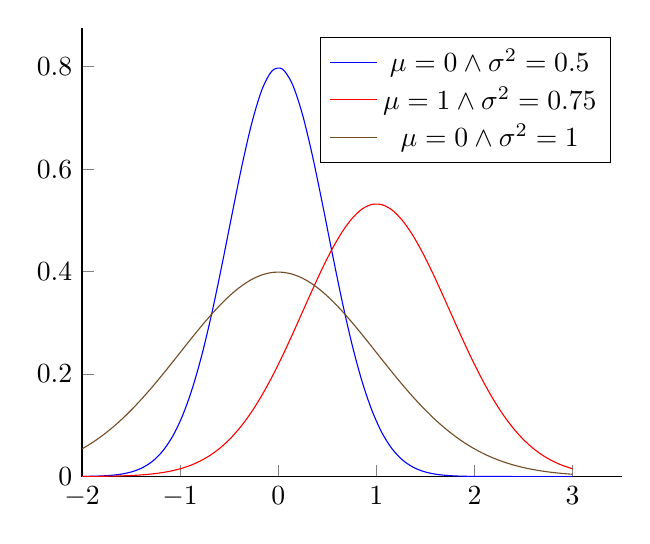
\begin{tikzpicture}
\pgfmathdeclarefunction{gauss}{2}{%
  \pgfmathparse{1/(#2*sqrt(2*pi))*exp(-((x-#1)^2)/(2*#2^2))}%
}

\begin{axis}[every axis plot post/.append style={
  mark=none,domain=-2:3,samples=50,smooth}, % All plots: from -2:2, 50 samples, smooth, no marks
  axis x line*=bottom, % no box around the plot, only x and y axis
  axis y line*=left, % the * suppresses the arrow tips
  enlargelimits=upper] % extend the axes a bit to the right and top
  \addplot {gauss(0,0.5)};
  \addlegendentry{$\mu=0 \land \sigma^{2}=0.5$}
  \addplot {gauss(1,0.75)};
  \addlegendentry{$\mu=1 \land \sigma^{2}=0.75$}
  \addplot {gauss(0,1)};
  \addlegendentry{$\mu=0 \land \sigma^{2}=1$}
\end{axis}
\end{tikzpicture}


%\end{document}